Underwater imaging capabilities are of great importance across a wide spectrum of disciplines, for instance, marine research and environmental analysis, where scientists dive to several reef locations with waterproof camera systems and quadrats to audit the abundance of coral over time \cite{universityofhawaiiPracticesScienceUnderwater}. Unmanned Underwater Vehicles (UUVs), a class of submersible vehicles, are pivotal in advancing these capabilities. With vast arrays of sensors and often remote-controlled or completely autonomous, UUVs enable the end user to conduct exploration missions of extended duration to analyse underwater environments with utmost accuracy even in the most hazardous conditions, impossible for direct human access. These benefits have caused UUVs to become common as a safer and cheaper alternative to manned vehicular operations in almost all underwater imaging-related applications, such as intelligence surveillance and reconnaissance in defence, defect and foreign object inspection in maritime, and oceanography and hydrography in marine research \cite{yannickallardUnmannedUnderwaterVehicle2014}.

When capturing images or recording video underwater, one would instantly notice the lack of light at greater sea depths. Coupling a high-power light source next to the camera resolves this issue to ensure a well-lit scene. However, this produces an adverse side-effect called backscatter, shown in Figure \ref{fig:backscatter}, where suspended particles in water scatter light in an inhomogeneous manner, reflecting the light emitted by the light source back into the camera, creating exceptionally bright spots and often saturating the image and degrading the quality \cite{sidharthshanmugamInitialReportMachine2024}. Albeit the existence of a few simple and universal techniques to mitigate backscatter, such as bringing the camera closer to the subject, fine-tuning the headlight position such that the subject is illuminated by only the edge of the light cone, or achieving perfect buoyancy to minimise disrupting sand, debris, and bubbles \cite{brentdurandEasyWaysEliminate2013}, they all lack viability for UUVs due the continuous and arbitrary propellor motion and the constant existence of backscatter-inducing debris floating throughout water bodies.

\begin{figure}[H]
    \centering
    \begin{subfigure}{.49\textwidth}
        \centering
        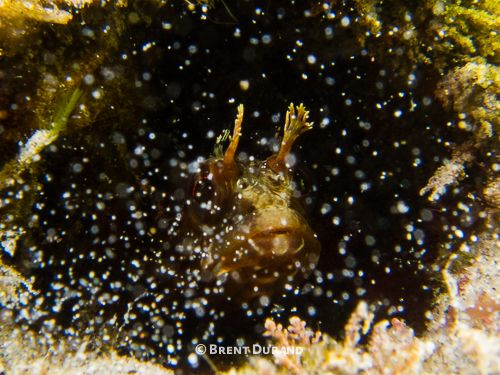
\includegraphics[width=1\linewidth]{assets/backscatter_article_durand2.jpg}
        \caption{}
        % \label{subfig:backscatter_durand}
    \end{subfigure}
    \hfill
    \begin{subfigure}{.49\textwidth}
        \centering
        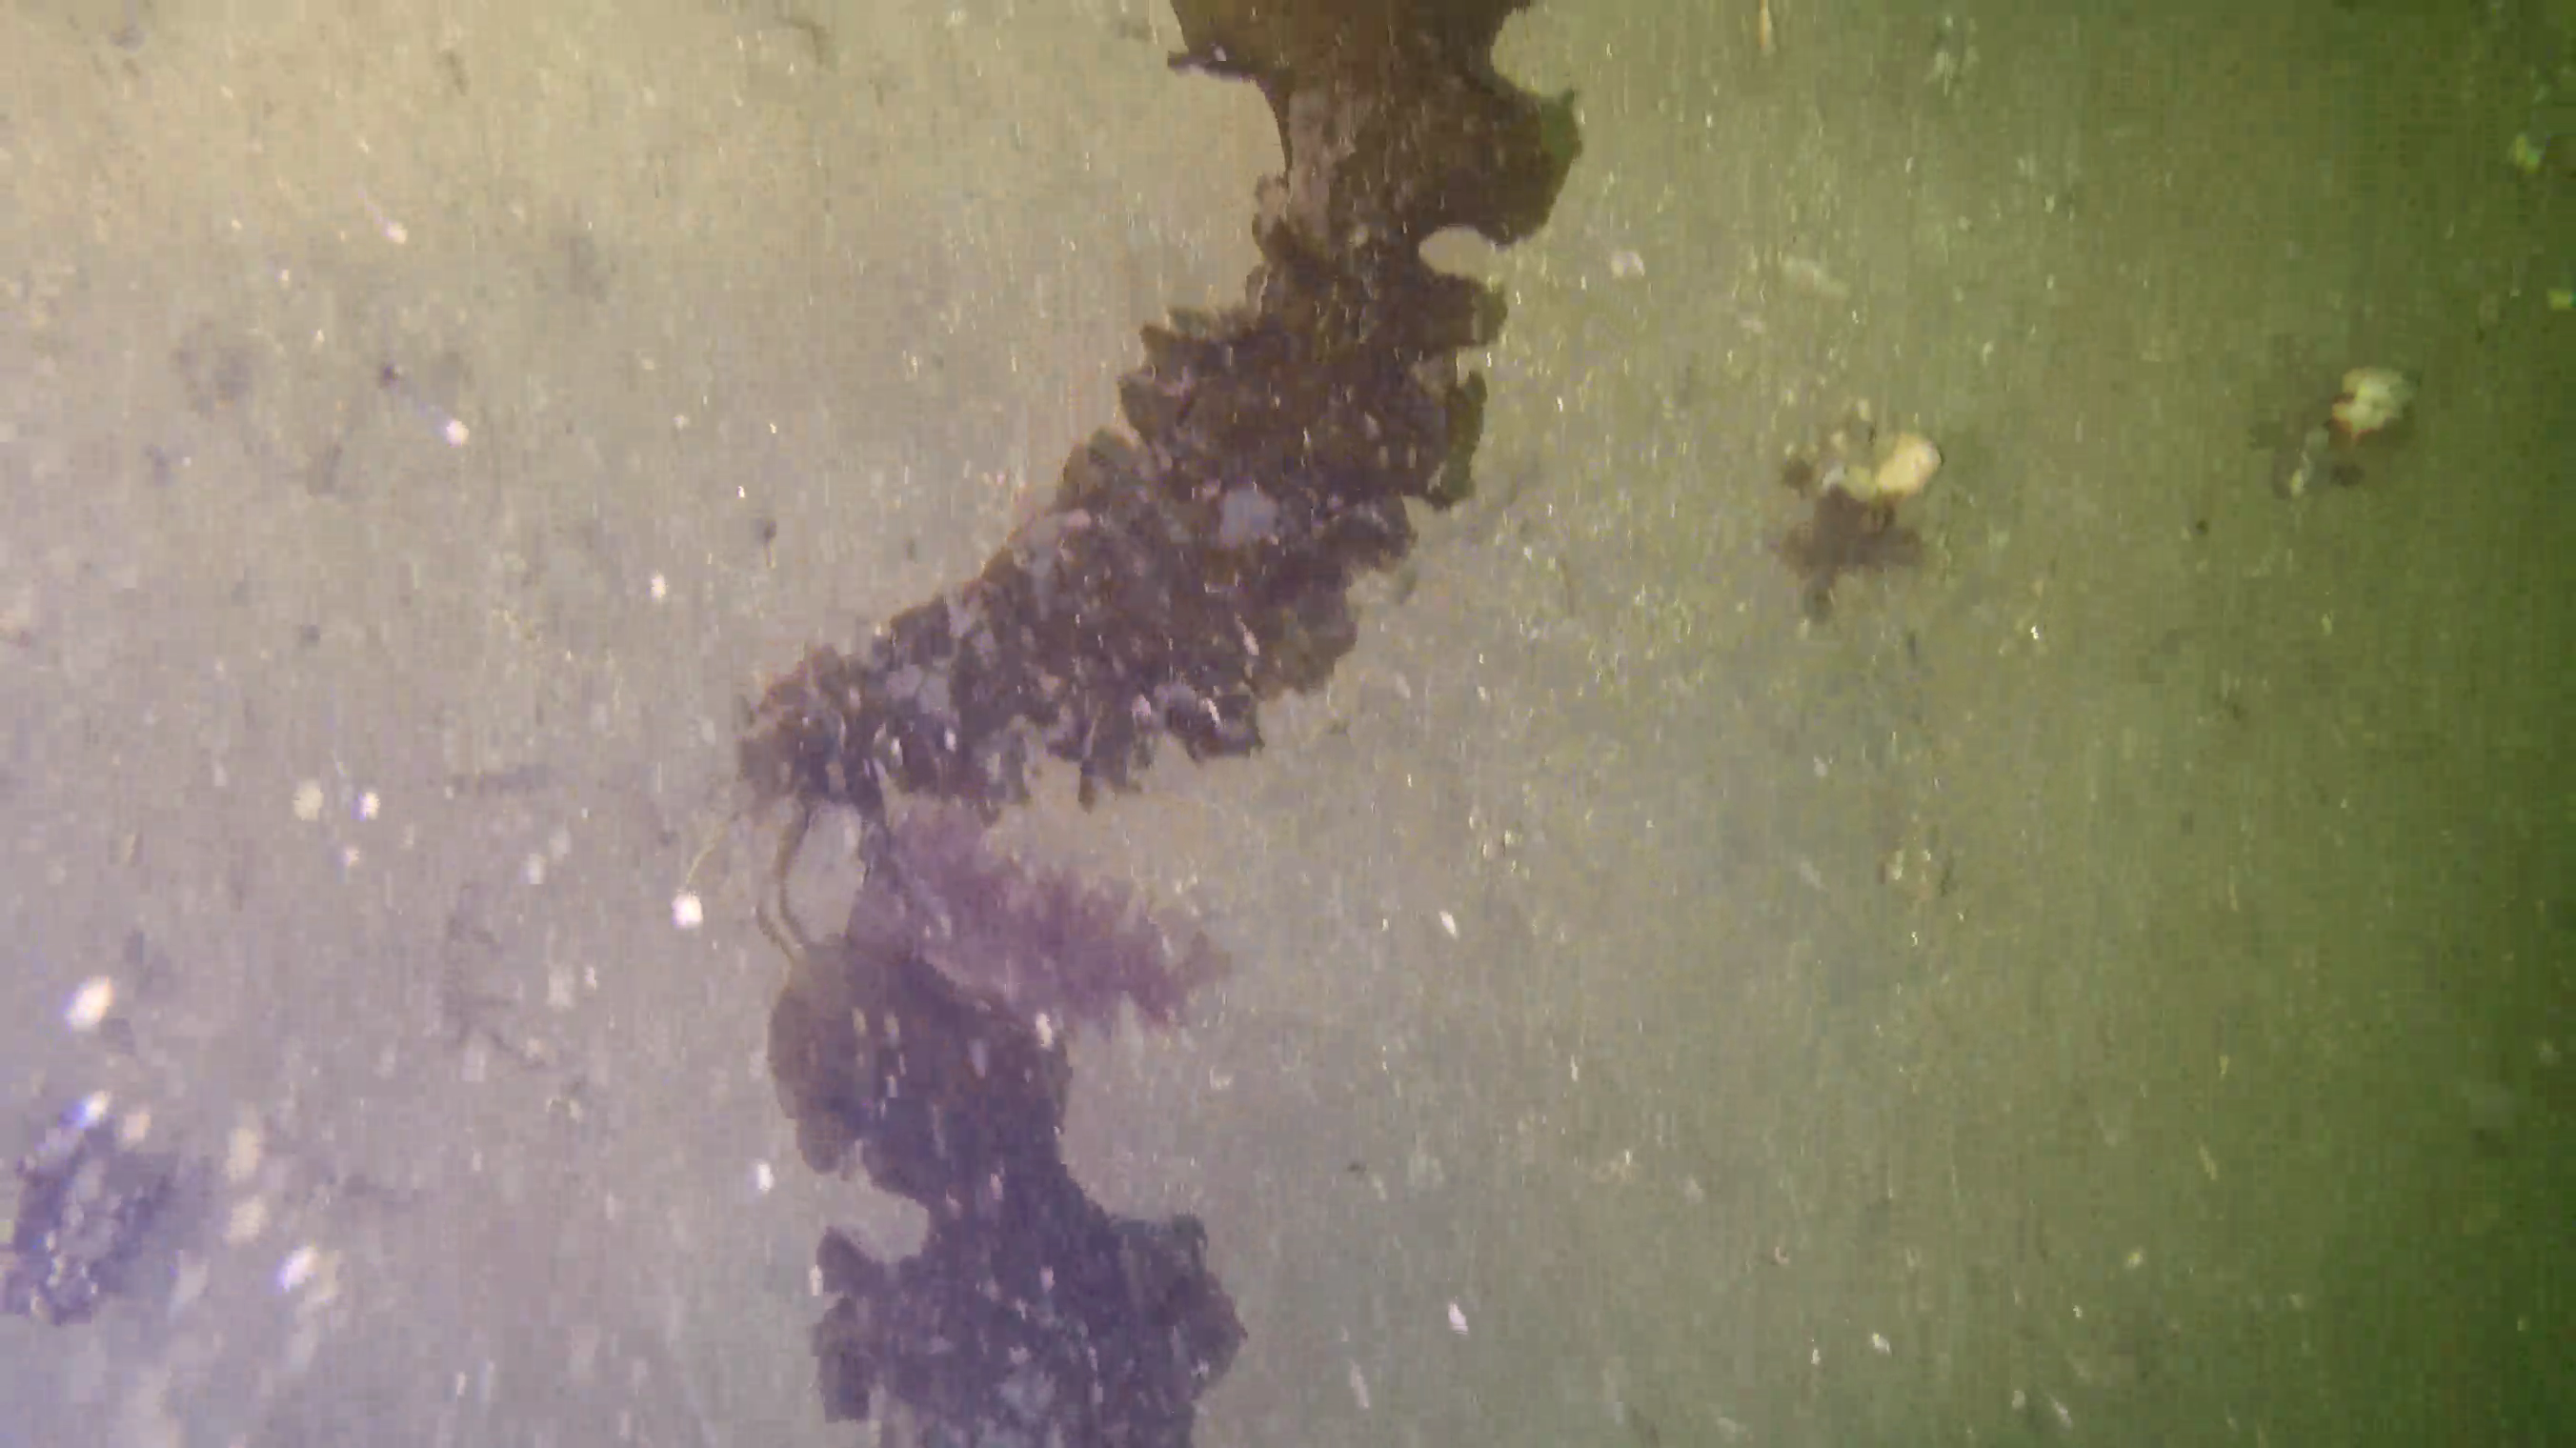
\includegraphics[width=1\linewidth]{assets/backscatter_test_vid.png}
        \caption{}
        % \label{subfig:backscatter_gopro}
    \end{subfigure}
    \caption{(a) Backscatter appears as the particles of sand drift between the aquatic animal and the camera, retrieved from \cite{brentdurandEasyWaysEliminate2013}. (b) A captured frame in GoPro footage from a UUV of the seabed with backscatter increasing as the propellors disrupt the sand.}
    \label{fig:backscatter}
\end{figure}

With a specialised camera sensor to capture fast-moving backscatter particles, a single-board computer processing frames using advanced machine vision technologies to detect backscatter, and a specialised projector to project selectively illuminated light patterns, the project's ultimate goal is to develop a novel backscatter-cancelling light source to aid the generation of high-quality underwater images in real-time, thus eliminating the requirement for a camera with better dynamic range compatibility to compensate for the bright regions from backscatter and lens flares. The first objective is to research architectures to develop a reliable backscatter detection system, tieing in with the second objective of researching methodologies to optimise for real-time to ensure predictability and stability, ensuring the projection of backscatter-cancelling light patterns with minimal and consistent latency.

Section \ref{background} summarises the information in related theoretical realms to form the foundation of the subsequent sections. Section \ref{design} first introduces the assumptions and requirements before detailing the high-level processes for both the lighting system and toolsets for testing. Section \ref{implementation} showcases the system and toolset implementations, which Section \ref{testing} then quantifies by evaluating the real-time performances. Section \ref{conclusion} reflects on these evaluations, including a reflection on project execution and a discussion of future work.
